 %&latex
\documentclass[smaller,a4paper]{beamer}
\usepackage{amsmath,amssymb,pdfsync,listings}
\usepackage{graphicx}
\usepackage{truncate}
%%\usepackage{mpmulti}
\usepackage{times}

\newcommand{\largenameref}[1]{\textbf{\huge{\nameref{#1}}}}
\newcommand{\largehyperlink}[2]{\textbf{\Large\hyperlink{#1}{#2} }}
\newcommand{\largehypertarget}[2]{\textbf{\color{red} \hypertarget{#1}{#2} }}
\newcommand{\Largehypertarget}[2]{\textbf{\Large \color{red} \hypertarget{#1}{#2} }}
\newcommand{\Int}[2]{\displaystyle{\int\limits_{#1}^{#2}}}      
\newcommand{\Sum}[2]{\displaystyle{\sum\limits_{#1}^{#2}}}      
\newcommand{\Myfoilheadskip}[1]{\begin{frame}\frametitle{#1}}
\newcommand{\trace}[2]{\left. #1 \right\rvert_{_{#2} }  }
\newcommand{\mtrx}[1]{\mathbf{#1}}
\newcommand{\vect}[1]{\mathbf{#1}}
\newcommand{\abs}[1]{\left|#1\right|}

\usepackage[english]{babel}

\begin{document}
\title{Galerkin/Linear Finite Elements Method in 1d, with non uniform coefficients}
\frame{\titlepage}

%%%%%%%%%%%%%%%%%%%%%%%%%%%%%%%%%%%%%%%%%%%%%%%%%%%%
\Myfoilheadskip{Problem Statement}%\hypertarget{targ:outline}{}
%%%%%%%%%%%%%%%%%%%%%%%%%%%%%%%%%%%%%%%%%%%%%%%%%%%%

We want to implement a solver for the 
following boundary value problem:

\begin{equation}\label{eq:formaforte}
\left\{
\begin{array}{l}
-(a(x) u^{\prime})^{\prime} = f(x) \qquad \mbox{in } (0,1)       \\
u(0)=u(1)=0       
\end{array}
\right.
\end{equation}

where the coefficients $a(x)$ and $f(x)$ are to be specified by the user at run time

\end{frame}
%%%%%%%%%%%%%%%%%%%%%%%%%%%%%%%%%%%%%%%%%%%%%%%%%%%%
\Myfoilheadskip{Weak Formulation}%\hypertarget{targ:outline}{}
%%%%%%%%%%%%%%%%%%%%%%%%%%%%%%%%%%%%%%%%%%%%%%%%%%%%

The weak form of equation \eqref{eq:formaforte} reads:
\begin{equation}\label{eq:formadebole}
\left\{
\begin{array}{l}
\text{find } u\in V=H_{0}^{1}(0,1) s.t.       \\[3mm]
-\Int{0}{1} (a(x)\ u')' \varphi \,dx  = \Int{0}{1} f(x) \cdot \varphi \,dx \quad \forall \varphi \in V
\end{array}
\right.
\end{equation}

Using integration by parts we get
\begin{equation*}
-\Int{0}{1} (a(x)\ u')' \varphi \,dx=\Int{0}{1} a(x)\ u' \varphi' \,dx- \trace{a(x)\ \varphi u'}{0}^{1}=\Int{0}{1} a(x)\ u' \varphi'  \,dx
\end{equation*}

\end{frame}

%%%%%%%%%%%%%%%%%%%%%%%%%%%%%%%%%%%%%%%%%%%%%%%%%%%%
\Myfoilheadskip{Galerkin Method}%\hypertarget{targ:outline}{}
%%%%%%%%%%%%%%%%%%%%%%%%%%%%%%%%%%%%%%%%%%%%%%%%%%%%

Let $V_{h}\subset V$ be a subspace of finite dimension $N_h$
and let $\{\varphi_{i}\}\subseteq V_{h}$ be a basis of $V_{h}$
\begin{equation}\label{eq:galerkin}
\left\{
\begin{array}{l}
\text{find } u_{h}\in V_{h} s.t.       \\[3mm]
\Int{0}{1} a(x) u_{h}' \varphi_{i}' \,dx  = \Int{0}{1} f(x) \cdot \varphi_{i} \,dx \quad \forall \varphi_{i} \in V_{h}
\end{array}
\right.
\end{equation}

We can express $u_{h}$ as a linear combination of basis vectors:
\begin{equation*}
u_{h} = \Sum{j=1}{N_h} u_{j}\varphi_{j} \Rightarrow u_{h}'= \Sum{j=1}{N_h} u_{j} \varphi' _{j}
\end{equation*}
\end{frame}

%%%%%%%%%%%%%%%%%%%%%%%%%%%%%%%%%%%%%%%%%%%%%%%%%%%%
\Myfoilheadskip{Galerkin Method}%\hypertarget{targ:outline}{}
%%%%%%%%%%%%%%%%%%%%%%%%%%%%%%%%%%%%%%%%%%%%%%%%%%%%

Equation \ref{eq:galerkin}$_{2}$ becomes:
\begin{equation*}
\Sum{j=1}{N_h} u_{j} \Int{0}{1} a(x)\ \varphi_{i}'\varphi_{j}' \,dx = \Int{0}{1}f(x)\ \varphi_{i} \,dx \quad i=1,\ldots,N_h
\end{equation*}

We therefore get a linear algebraic system of the form
$$
\mtrx{A} \vect{u} = \vect{f},
$$
where
$$
A_{ij}=  \Int{0}{1} a(x)\ \varphi_{i}'\varphi_{j}' \,dx, \,\, f_{i}= \Int{0}{1} f(x)\ \varphi_{i} \,dx
$$
and the vector of unknowns $\vect{u}$ is formed by the coefficients of the expansion of $u_{h}$ w.r.t. the basis $\{\varphi_{i}\}$

\end{frame}

%%%%%%%%%%%%%%%%%%%%%%%%%%%%%%%%%%%%%%%%%%%%%%%%%%%%
\Myfoilheadskip{Linear Finite Elements}%\hypertarget{targ:outline}{}
%%%%%%%%%%%%%%%%%%%%%%%%%%%%%%%%%%%%%%%%%%%%%%%%%%%%

Let us define a \emph{triangulation} of the interval $(0,1)$
\begin{center}
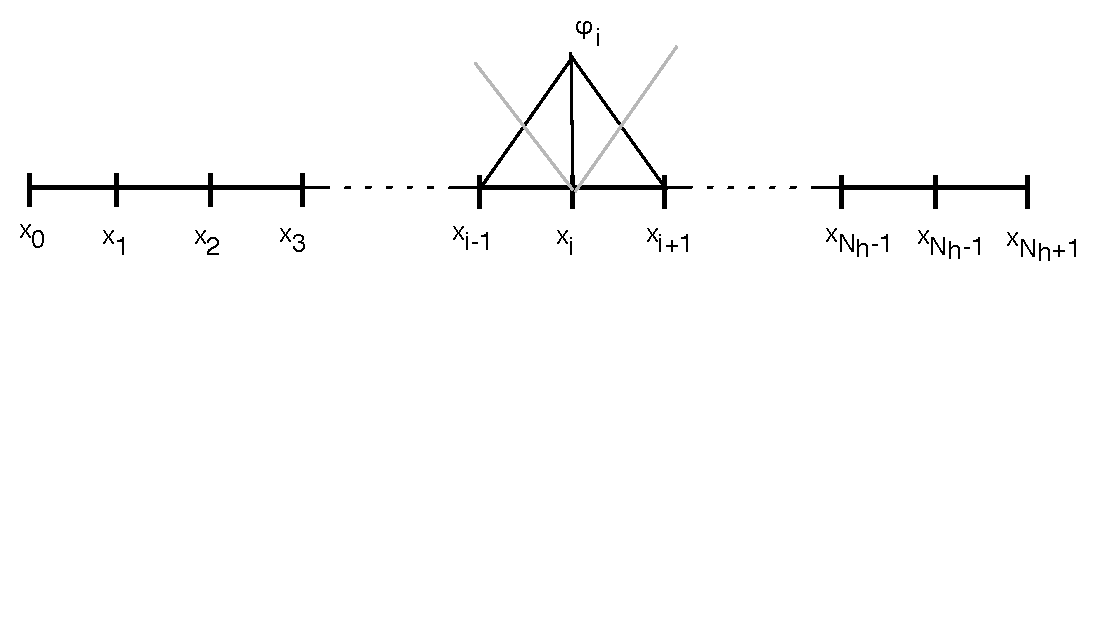
\includegraphics[width=.5\linewidth]{mesh}
\end{center}

Let as choose as the finite dimensional space $V_{h}$ the
set of functions that are continuous in $(0,1)$
and are degree-$1$ polynomials ({\it i.e.}, affine functions) in each subintervall.

the canonical basis for $V_{h}$ is gicen by:

$$
\{\varphi_{i}\}=\{\varphi_{i} \in V_{h} \, t.c.\, \varphi_{i}(x_{j})=\delta_{ij} \}
$$

\end{frame}

%%%%%%%%%%%%%%%%%%%%%%%%%%%%%%%%%%%%%%%%%%%%%%%%%%%%
\Myfoilheadskip{Implementation of the Linear FEM I}%\hypertarget{targ:outline}{}
%%%%%%%%%%%%%%%%%%%%%%%%%%%%%%%%%%%%%%%%%%%%%%%%%%%%

Using the local support property of the Finite Element basis
$\varphi_{i}(x) \neq 0 $ solo se $x\in(x_{i-1},x_{i+1})$
we get
$$
A_{ij}=\left\{
\begin{array}{l}
0 \,\, \mbox{if } \abs{i-j} > 1 \\[2mm]
\Int{x_{i-1}}{x_{i}} a(x)\ \varphi{'_{i}}^{2} +
\Int{x_{i}}{x_{i+1}} a(x)\ \varphi{'_{i}}^{2}
 \,\, \mbox{if } i=j \\[4mm]
\Int{x_{i-1}}{x_{i}} a(x)\ \varphi'_{i}\varphi'_{i-1} \,\, \mbox{if } j=i-1 \\[4mm]
\Int{x_{i}}{x_{i+1}} a(x)\ \varphi'_{i}\varphi'_{i+1} \,\, \mbox{if } j=i+1 
\end{array}
\right.
$$

\begin{itemize}
\only<1>{\item the non zero terms in the matrix are $N_h+2*(N_h-1)$ (the matrix is therefore sparse and tridiagonal)}
\only<2>{\item each entry in the matrix is given by a sum of (few) integrals each computed on only one subinterval}
\only<3>{\item the integrals cannot be computed exactly in general, we need to use a \emph{quadrature rule}}
\end{itemize}

\end{frame}

%%%%%%%%%%%%%%%%%%%%%%%%%%%%%%%%%%%%%%%%%%%%%%%%%%%%
\Myfoilheadskip{Implementation of the Linear FEM II}%\hypertarget{targ:outline}{}
%%%%%%%%%%%%%%%%%%%%%%%%%%%%%%%%%%%%%%%%%%%%%%%%%%%%

To assemble $\mtrx{A}$, we decompose the intervals of $(0,1)$ into integrals on subintervals: 
$$
A_{ij}=\Int{0}{1} a(x)\ \varphi'_{i}\varphi' _{j} \,dx= \Sum{k=1}{N_h+1} \Int{x_{k-1}}{x_{k}} a(x)\ \varphi'_{i}\varphi' _{j}\,dx
$$

We can then use the following algorithm for assembling $\mtrx{A}$:

\begin{enumerate}
\item Initialize all elements of $\mtrx{A}$ to $0$
\item Compute integrals on subintervals
\item Compute entries od $\mtrx{A}$ as sums of the partial integrals
\end{enumerate}

This is unnecessary for this simple case but has advantages in more complex situations we will
discuss later:
\begin{enumerate}
\item Extension to different bases
\item Extension to multiple space dimensions
\item Parallel computing
\end{enumerate}
\end{frame}

%%%%%%%%%%%%%%%%%%%%%%%%%%%%%%%%%%%%%%%%%%%%%%%%%%%%
\Myfoilheadskip{Implementation of the Linear FEM III}%\hypertarget{targ:outline}{}
%%%%%%%%%%%%%%%%%%%%%%%%%%%%%%%%%%%%%%%%%%%%%%%%%%%%

In each subinterval $(x_{k-1},x_{k})$ there are four integrals $\neq 0$ which 
need to be computed, they are usually arranged into a \emph{local matrix}:

$$
\mtrx{A_{loc}}=
\left[\begin{array}{cc}
i=k-1,j=k-1 & i=k-1,j=k \\[.1cm]
i=k,j=k-1 & i=k,j=k 
\end{array}\right]
$$

\null

\noindent 
$A_{loc_{11}}$ will then be added to $A_{k-1,k-1}$  \\
$A_{loc_{12}}$ will then be added to $A_{k-1,k}$ etc...

\null

this process is called assembly of the coefficient matrix

\end{frame}

\begin{frame}\frametitle{Exercise}
\begin{itemize}
\item adapt the fem1d code to allow the user to specify the coefficients $a(x)$ and $f(x)$ at runtime
\begin{itemize}
\item use the trapezoidal rule to compute integrals
\item use muparser to parse the function provided by the user
\end{itemize}
\item adapt the fem1d code to allow the user to specify the quadrature rule at runtime
\end{itemize}
\end{frame}

\begin{frame}[fragile]
\frametitle{Implementation in {\tt C++} }
\only<1-2>{file {\tt fem1d.h}}
\only<3-6>{file {\tt fem1d.cpp}}
\tiny
\only<1>{\lstinputlisting[language=C++, firstline=1, firstnumber=1, lastline=35, numbers=left, numberstyle=\tiny\color{gray}]{../fem1d-0.7/fem1d.h}}
\only<2>{\lstinputlisting[language=C++, firstline=35, firstnumber=35, lastline=70, numbers=left, numberstyle=\tiny\color{gray}]{../fem1d-0.7/fem1d.h}}
\only<3>{\lstinputlisting[language=C++, firstline=1, firstnumber=1, lastline=35, numbers=left, numberstyle=\tiny\color{gray}]{../fem1d-0.7/fem1d.cpp}}
\only<4>{\lstinputlisting[language=C++, firstline=35, firstnumber=35, lastline=70, numbers=left, numberstyle=\tiny\color{gray}]{../fem1d-0.7/fem1d.cpp}}
\only<5>{\lstinputlisting[language=C++, firstline=70, firstnumber=70, lastline=105, numbers=left, numberstyle=\tiny\color{gray}]{../fem1d-0.7/fem1d.cpp}}
\only<6>{\lstinputlisting[language=C++, firstline=105, firstnumber=105, lastline=120, numbers=left, numberstyle=\tiny\color{gray}]{../fem1d-0.7/fem1d.cpp}}
\end{frame}

\end{document}